\documentclass{article}
\usepackage{assignment_preamble}

\title{Lab 5}
\author{Ravi Kini}
\date{December 15, 2023}

\begin{document}

\maketitle

\repository{https://github.com/ravidosa/notes/tree/main/academics/assignments/code/phy112l_lab5}

\problem
The modified Ising model has $S_i = -1, 0, 1$. A $4 \times 4$ lattice then has $3^{4 \cdot 4} = 3^{16} = 43046721$ possible states. At high temperatures, all microstates are equally accessible, so as $T \to \infty$, $S \to \ln 3^{16} = 16\ln 3 \approx 17.578$. At low temperatures, only the lowest energy state is accessible. There are two microstates where the system is in the state (all up and all down) with energy $-1 \cdot \left(4 \cdot \left(4 - 1\right) + \left(4 - 1\right) \cdot 4\right) = -24$, so as $T \to 0$, $S \to \ln 2 \approx 0.693$.

\clearpage

\problem
The transition temperature for this model is likely less than that of the Ising model. The average energy of this model is less negative than that of the Ising model; for a given energy, the number of states with that energy is at least that of the Ising model, as unoccupied sites do not add to the energy. The less negative an energy is, the more ways there are to produce a state with that energy, as there is more "room" to have unoccupied sites. Since $\langle E\rangle$ increases, decreasing the absolute value, and $S$ increases, $T_c$ must decrease to keep the balance.

\clearpage

\problem
Figure \ref{fig:fig1} is a plot of $\langle E \rangle$ vs. $T$ for $J = 1$ and $N = 3 \times 3$. As $T$ increases, the average energy increases.
\begin{figure}[!htb]
    \centering
    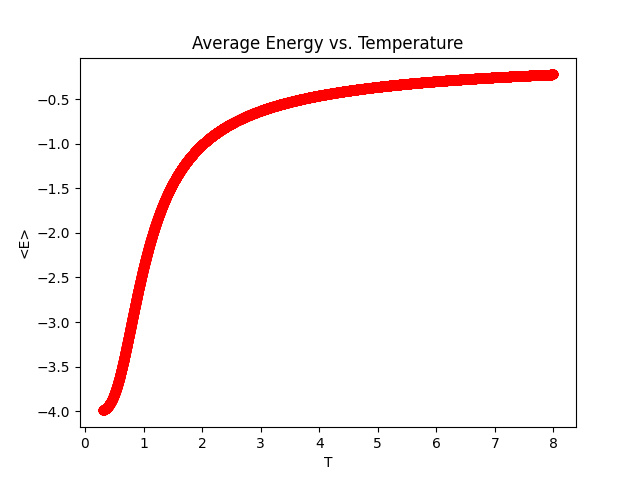
\includegraphics[width=0.75\textwidth]{../code/phy112l_lab5/5-3.png}
    \caption{Plot of average energy vs. temperature ($J = 1, N = 3 \times 3$).}
    \label{fig:fig1}
\end{figure}

\clearpage

\problem
Figure \ref{fig:fig2} is a plot of $\langle E \rangle$ vs. $T$ for $J = 1$ and $N = 3 \times 3$ with $3$ vacancies. As $T$ increases, the average energy increases. At low temperatures, only the lowest energy state is accessible. With no constraint on the number of vacancies, the lowest energy states have energy $-1 \cdot \left(3 \cdot \left(3 - 1\right) + \left(3 - 1\right) \cdot 3\right) = -12$. With the number of vacancies constrained to exactly three, we seek to minimize the number of interactions that involve a vacancy. Placing a vacancy in the corner produces two interactions with a vacancy, placing a vacancy on a non-corner edge produces three interactions with a vacancy, placing a vacancy on neither a corner nor an edge produces four interactions with a vacancy, and placing a vacancy next to $n$ vacancies remove $n$ interactions with a vacancy due to overcounting. We first place a vacancy in the corner, producing two interactions with a vacancy. Placing a vacancy in an edge next to this corner produces two more interactions with a vacancy. Placing a vacancy along the edge next to the previous vacancy produces one more interaction with a vacancy, as that site is also a corner, for a minimal total of five interactions with a vacancy. The lowest energy states then have energy $-1 \cdot \left(3 \cdot \left(3 - 1\right) + \left(3 - 1\right) \cdot 3 - 5\right) = -7$.
\begin{figure}[!htb]
    \centering
    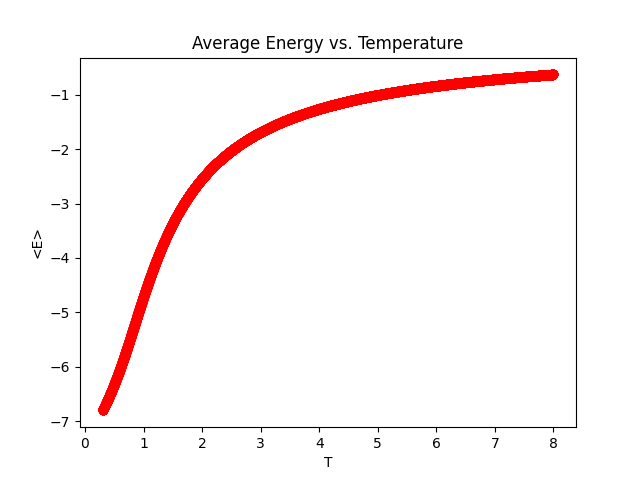
\includegraphics[width=0.75\textwidth]{../code/phy112l_lab5/5-4.png}
    \caption{Plot of average energy vs. temperature ($J = 1, N = 3 \times 3$, $3$ vacancies).}
    \label{fig:fig2}
\end{figure}

\clearpage

\problem
Figure \ref{fig:fig3} is a plot of $\langle E \rangle$ vs. $T$ for $J = 1$ and $N = 4 \times 4$. As $T$ increases, the average energy increases.
\begin{figure}[!htb]
    \centering
    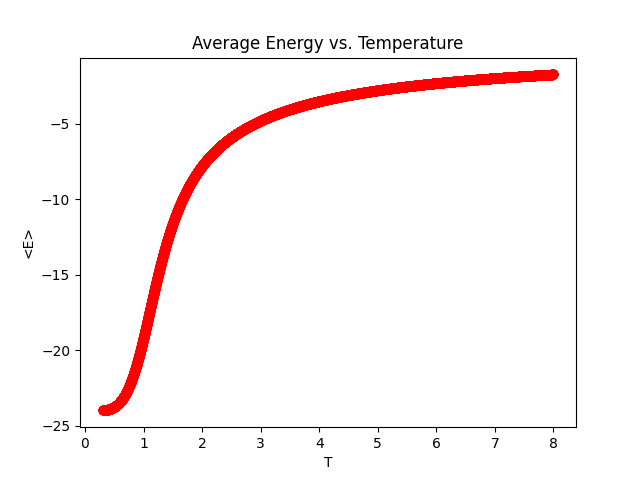
\includegraphics[width=0.75\textwidth]{../code/phy112l_lab5/5-5.png}
    \caption{Plot of average energy vs. temperature ($J = 1, N = 4 \times 4$).}
    \label{fig:fig3}
\end{figure}

\end{document}